\documentclass[a4paper,10pt]{article}
\usepackage[utf8]{inputenc}
\usepackage{tikz}

%opening
\title{}
\author{}

\begin{document}

\maketitle

\begin{abstract}

\end{abstract}

\section{}
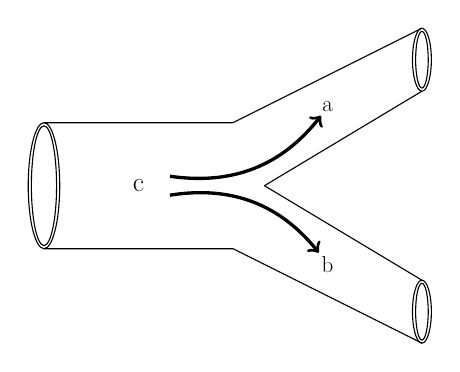
\begin{tikzpicture}[scale=0.4, transform shape]
\draw circle (0.5cm and 2cm) (0,2) -- (6,2) (0,-2) -- (6,-2);
\draw circle (0.4cm and 1.9cm);
\draw (6,2) -- (12,5) (7,0) -- (12,3);
\draw (12,4) circle (0.3 and 1);
\draw (12,4) circle (0.2 and 0.9);
\draw (6,-2) -- (12,-5) (7,0) -- (12,-3);
\draw (12,-4) circle (0.3 and 1);
\draw (12,-4) circle (0.2 and 0.9);
\node (node_C) at (3,0) {\Huge{c} };
\node (node_a) at (9,2.5) {\huge{a}};
\node (node_b) at (9,-2.5) {\huge{b}};
\path[very thick,->] (4,0.3) edge [bend right] (node_a);
\path[very thick,->] (4,-0.3) edge [bend left] (node_b);

\end{tikzpicture}

\end{document}
